\section{信号流图}

\subsection{信号流图}

\begin{BoxDefinition}[信号流图]
    信号流图是由结点和有向线段组成的几何图形。可以简化系统的表示并便于计算系统函数。
\end{BoxDefinition}

\begin{BoxDefinition}[信号流图的常用术语]*
    结点表示系统中的变量或信号的点。

    连接两个结点之间的有向线段称为支路,支路上的权值又称支路增益,是两结点间的系统函数(转移函数)。

    源点是只有出支路的结点,又称输入结点;汇点是只有入支路的结点,又称输出结点;有入有出的结点称为混合结点。

    沿箭头方向从一个结点到其他结点的路径(多个支路)称为路径。

    如果通路与任一结点相遇不多于一次,则称为开通路;闭合的路径称为闭通路,又称回路或环;相互没有公共结点的回路,称为不接触回路;只有一个结点和一条支路的回路称为自回路。

    前向通路是从源点到汇点的开通路。

    前向通路增益和回路增益是通路中各支路增益的乘积。
\end{BoxDefinition}

\begin{BoxProperty}[信号流图的基本性质]
    信号只能沿支路箭头方向传输,且支路的输出=该支路的输入与支路增益的乘积。

    当结点有多个输入时,该结点将所有的输入支路的信号相加,并将和信号传输给所有与该结点相连的输出支路。

    混合结点可通过增加一个增益为$1$的出支路而变为汇点。
\end{BoxProperty}

系统框图与信号流图的转换如下

\begin{Figure}[系统框图与流图的转换]
    \begin{FigureSub}[系统框图]
        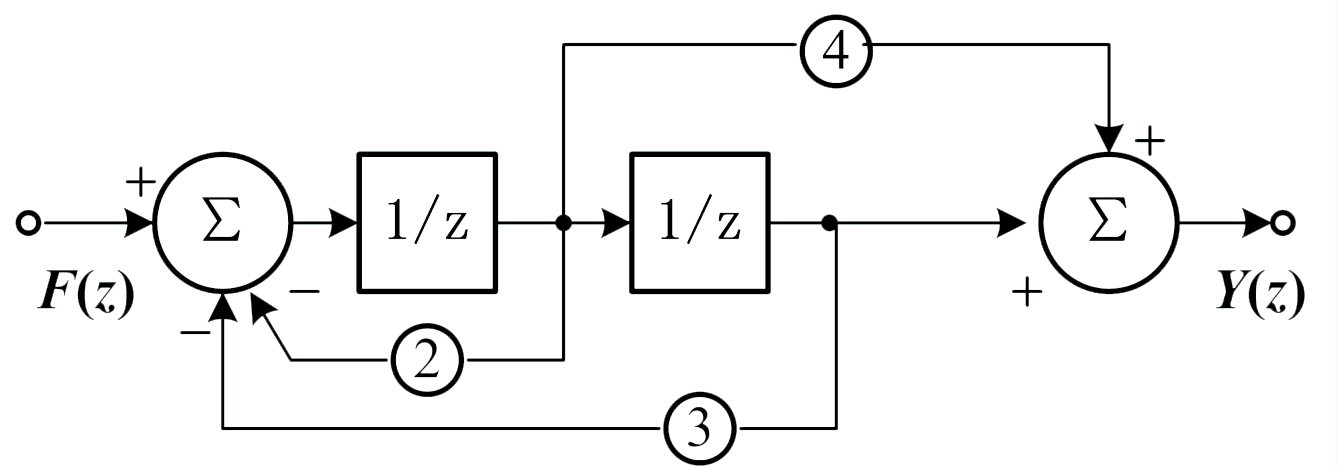
\includegraphics[width=75mm]{img/7.2.png}
    \end{FigureSub}
    \begin{FigureSub}[信号流图]
        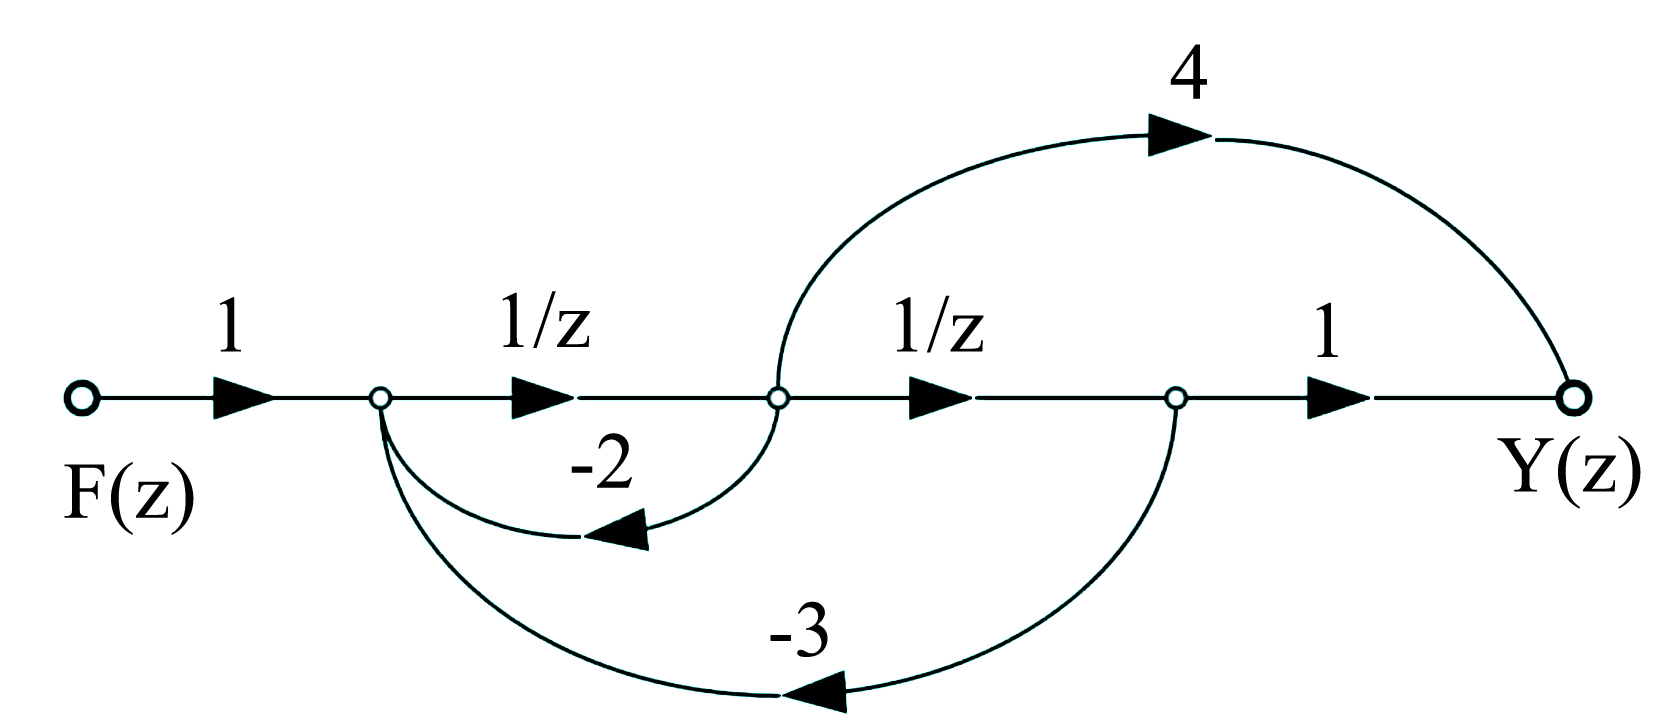
\includegraphics[width=75mm]{img/7.2-bn.png}
    \end{FigureSub}
\end{Figure}

注意加法器前引入了增益为$1$的支路。

\begin{BoxProperty}[信号流图的简化]
    \begin{Figure}[支路串联]
        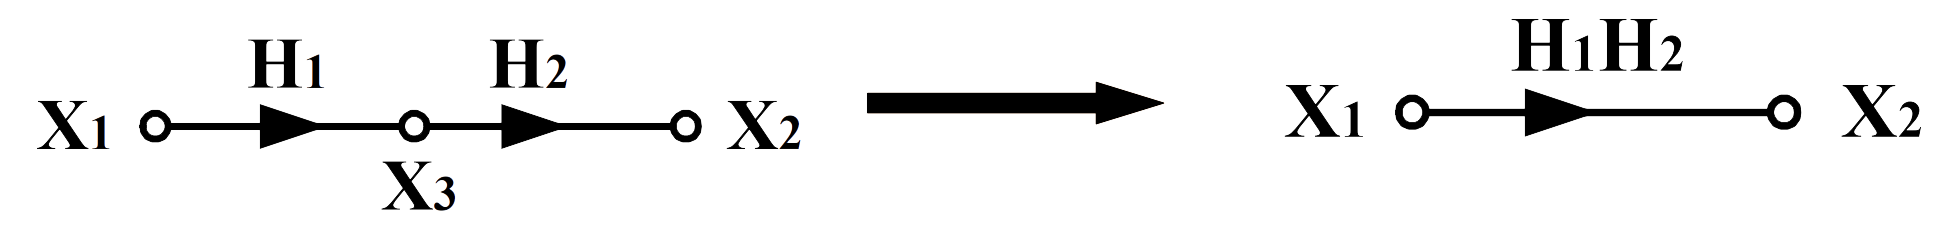
\includegraphics[width=60mm]{img/7.3-a.png}
    \end{Figure}
    支路串联
    \begin{Equation}
        X_2 = H_2X_3 = H_1H_2X_1
    \end{Equation}
    \begin{Figure}[支路并联]
        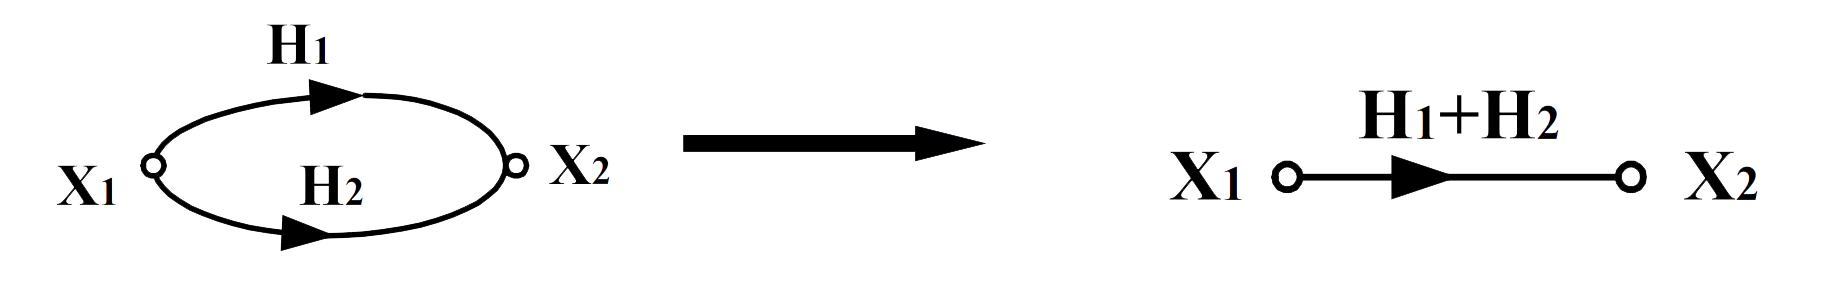
\includegraphics[width=60mm]{img/7.4.png}
    \end{Figure}
    支路并联
    \begin{Equation}
        X_2 = H_1X_1 + H_2X_1 = (H_1+H_2)X_1
    \end{Equation}
    \begin{Figure}[混联]
        \begin{FigureSub}[多入支路单出支路混联]
            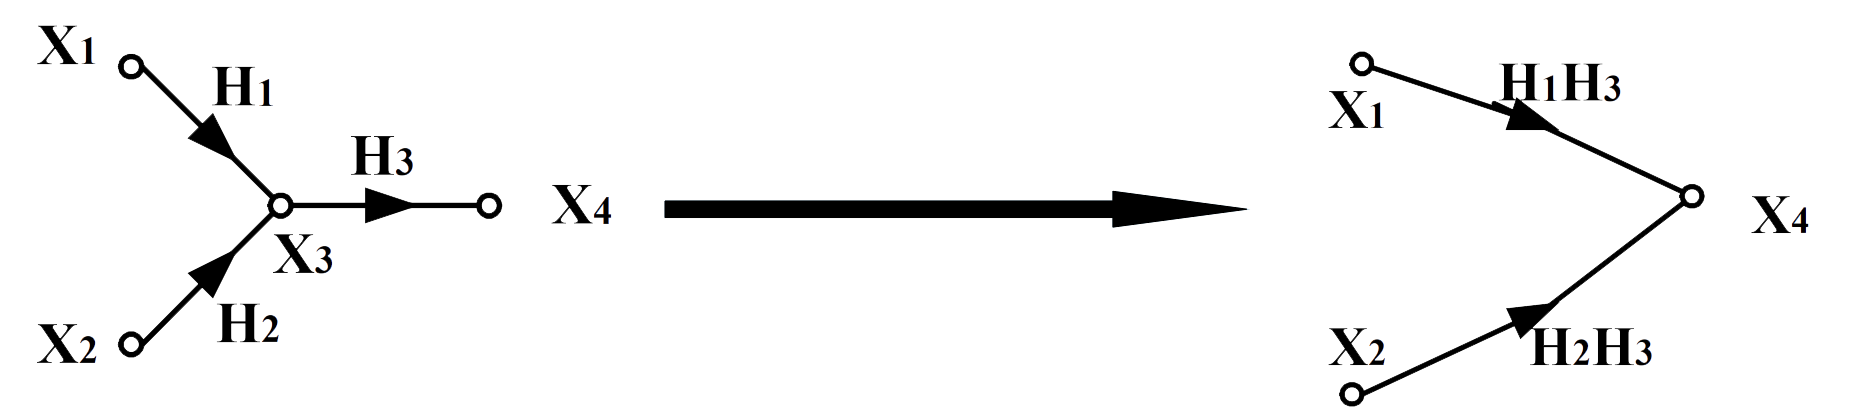
\includegraphics[width=60mm]{img/7.5-a.png}
        \end{FigureSub}
        \begin{FigureSub}[多出支路单入支路混联]
            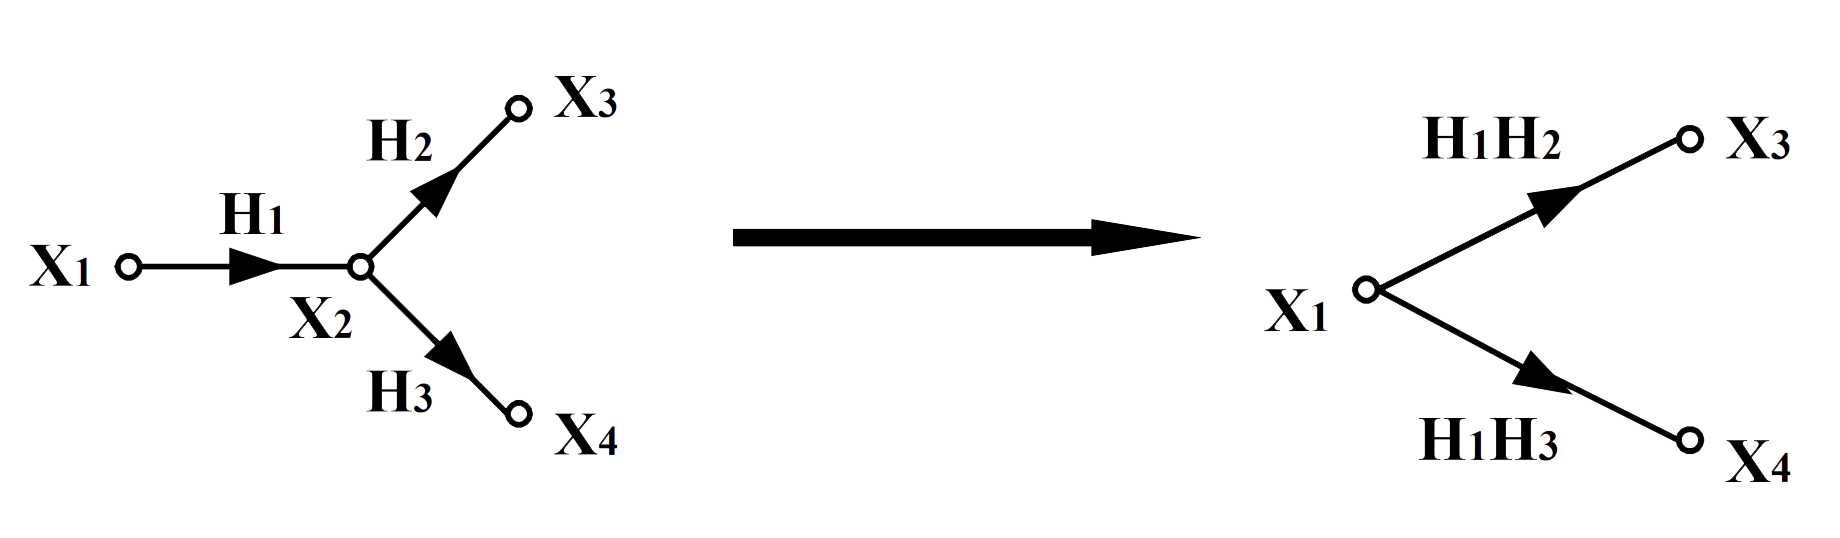
\includegraphics[width=60mm]{img/7.5-b.png}
        \end{FigureSub}
    \end{Figure}
    多入支路单出支路混联
    \begin{Equation}
        H_4=H_3X_3 = H_3(H_1X_1+H_2X_2) = H_1H_3X_1 + H_2H_3X_2
    \end{Equation}
    多出支路单入支路混联
    \begin{Equation}
        X_3 = H_2X_2 = H_1H_2X_1
    \end{Equation}
    \begin{Equation}
        X_4 = H_3X_2 = H_1H_3X_1
    \end{Equation}
    \begin{Figure}[自环的消除]
        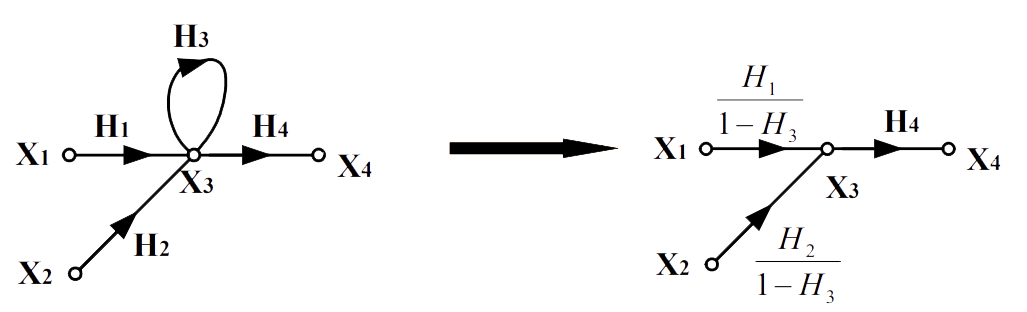
\includegraphics[width=60mm]{img/7.6.png}
    \end{Figure}
    自环的消除
    \begin{Equation}
        H_3 = H_1X_1 + H_2X_2 + H_3X_3 = \frac{H1}{1-H_3}X_1 + \frac{H_2}{1-H_3}X_2
    \end{Equation}
\end{BoxProperty}

信号流图的化简过程不一定相同,但结果一定相同。

\subsection{梅森公式}

\begin{BoxFormula}[梅森公式]
    系统函数$H(\cdot)$记为$H$,梅森公式为
    \begin{Equation}
        H = \frac{1}{\Delta} \sum\limits_{i} p_i \Delta_i
    \end{Equation}
    其中$\Delta$称为特征行列式,其表达式
    \begin{Equation}
        \Delta = 1 - \sum\limits_{j} L_j + \sum\limits_{m,n}L_mL_n - \sum\limits_{p,q,r}L_pL_qL_r + \dots
    \end{Equation}
    其中$\sum\limits_{j} L_j$为不同回路增益之和。

    $\sum\limits_{m,n}L_mL_n$为两两不接触\footnote{即在所有回路里两回路没有公共结点}的回路的乘积增益之和。

    $\sum\limits_{p,q,r}L_pL_qL_r$为三三不接触的回路的乘积增益之和。

    $p_i$是第$i$条前向通路的增益,$\Delta_i$是与第$i$条前向通路不接触的子图的特征行列式,又叫前向通路的余因子。
\end{BoxFormula}

使用梅森公式根据信号流图求解系统函数步骤:

\begin{itemize}
    \item 列出所有回路的增益,符号$L_j$
    \item 求特征行列式
    \item 列出所有前向通路的增益,符号$p_i$
    \item 求各前向通路的余因子$\Delta_i$
\end{itemize}